% -*- coding: utf-8; ispell-dictionary: "french"; -*-


%-------------------------------
% Chapter 4 - Exemples et Tests
%-------------------------------


Dans cette partie, trois exemples sont développés, depuis l'écriture du
composant avec Scade jusqu'à la sortie du couple de machines B correspondant.

\section{Bound}

Ce composant a déjà été décrit dans le chapitre 1. La planche Scade et la
version textuelle du composant sont les suivantes:

\begin{figure}[h]
\begin{center}
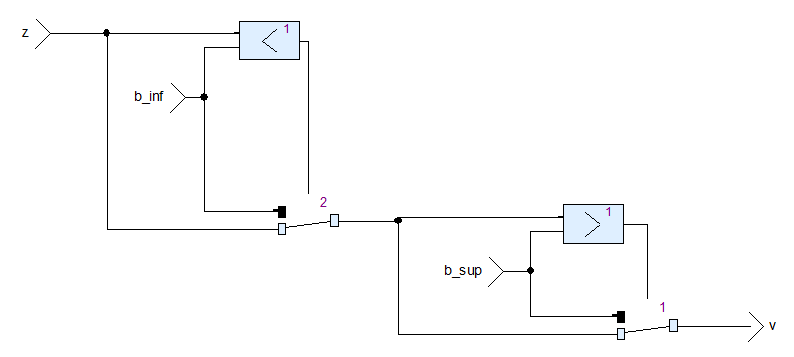
\includegraphics[scale=0.8]{1_bound.png}
\end{center}
\caption{Version graphique du noeud bound}
\end{figure}

\begin{figure}[h]
\begin{center}
\begin{footnotesize}
\begin{verbatim}
node bound(b_sup : int; z : int; b_inf : int) returns (v : int)
var
  _L7 : int;
  _L6 : bool;
  _L5 : int;
  _L4 : int;
  _L3 : bool;
  _L2 : int;
  _L1 : int;
let
  v= _L5;
  _L1= z;
  _L2= b_inf;
  _L3= _L7 > _L4;
  _L4= b_sup;
  _L5= if _L3 then (_L4) else (_L7);
  _L6= _L1 < _L2;
  _L7= if _L6 then (_L2) else (_L1);
  assume A_1 : b_inf <= 2000 and b_inf >= -2000;
  assume A_2 : b_sup <= 2000 and b_sup >= -2000;
  assume A_3 : z <= 2000 and z >= -2000;
  guarantee G_v : v <= 2000 and v >= -2000;
tel
\end{verbatim}
\end{footnotesize}
\end{center}
\caption{Version textuelle du noeud bound}
\end{figure}

\newpage

\noindent
Le couple de machines engendré par la traduction est le suivant.\\

\begin{center}
\begin{footnotesize}
\setlength{\columnseprule}{0.05cm}
\begin{multicols}{2}
\begin{alltt}
MACHINE Bound

OPERATIONS

vv \(\leftarrow\) bound(b_sup, zz, b_inf) =
 PRE
   zz \(\in\) INT & zz <= 2000 & zz >= -2000 &
   b_sup \(\in\) INT & b_sup <= 2000 & 
            b_sup >= -2000 &
   b_inf \(\in\) INT & b_inf <= 2000 & 
            b_inf >= -2000
 THEN
   vv \(\in\): \{ ii | ii \(\in\) INT & ii <= 2000 & 
            ii >= -2000 \}
 END 
END
\end{alltt}
\columnbreak
\begin{alltt}
IMPLEMENTATION Bound_i
REFINES Bound

OPERATIONS

vv \(\leftarrow\) bound(b_sup, zz, b_inf) =
 VAR L7, L6, L5, L4, L3, L2, L1 IN
   L4 := b_sup; 
   L2 := b_inf; 
   L1 := zz; 
   L6 := bool(L1 < L2); 
   IF L6 = TRUE THEN L7 := L2 ELSE L7 := L1 END; 
   L3 := bool(L7 > L4); 
   IF L3 = TRUE THEN L5 := L4 ELSE L5 := L7 END; 
   vv := L5
 END 
END
\end{alltt}
\end{multicols}
\end{footnotesize}
\end{center}



\newpage

\section{Integr}

Le noeud Integr a été présenté dans le chapitre 2. Les versions graphiques et
textuelles du composant sont les suivantes:

\begin{figure}[h]
\begin{center}
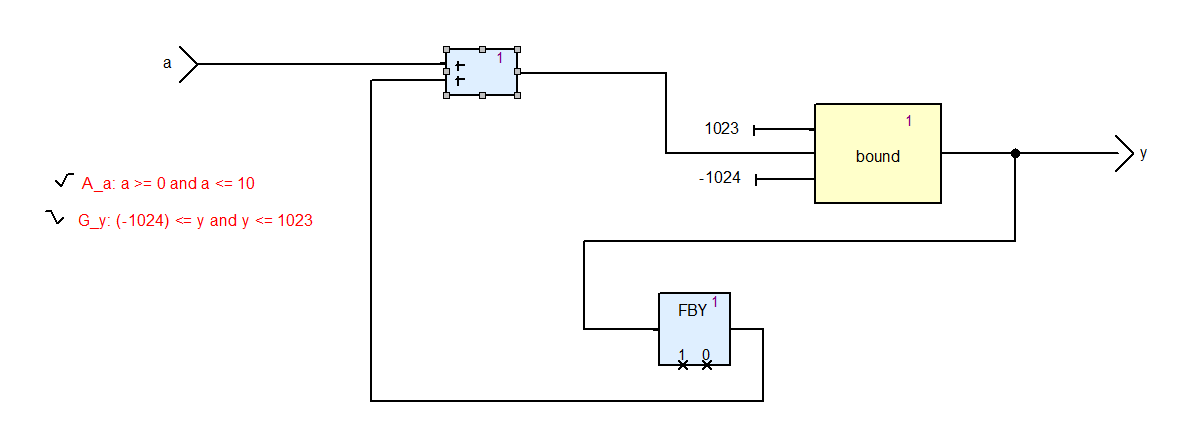
\includegraphics[scale=0.6]{4_integr.png}
\end{center}
\caption{Version graphique du noeud integr}
\end{figure}

\begin{figure}[h]
\begin{center}
\begin{small}
\begin{verbatim}
node integr(a : int) returns (y : int)
var
  _L7 : int;
  _L6 : int;
  _L5 : int;
  _L4 : int;
  _L3 : int;
  _L8 : int;
let
  _L3= 1023;
  _L4= a;
  y= _L8;
  _L5= - 1024;
  _L6= fby(_L8; 1; 0);
  _L7= _L4 + _L6;
  assume A_a : a >= 0 and a <= 10;
  guarantee G_y : - 1024 <= y and y <= 1023;
  _L8= #1 bound(_L3, _L7, _L5);
tel
\end{verbatim}
\end{small}
\end{center}
\caption{Version textuelle du noeud integr}
\end{figure}

On peut remarquer la présence d'un \emph{pragma} devant l'appel du composant
bound, symbolisé par un "\#" suivi d'un caractère numérique. Ces pragmas sont des
commentaires spéciaux utilisés par Scade, qui ne nous serons pas utiles. Ils
sont ignorés dans le processus de traduction.

\newpage
\noindent
Le couple de machines B engendré est le suivant:

\begin{center}
\begin{small}
\setlength{\columnseprule}{0.05cm}
\begin{multicols}{2}
\begin{alltt}
MACHINE Integr

OPERATIONS

yy \(\leftarrow\) integr(aa) =
 PRE
   aa \(\in\) INT & aa >= 0 & aa <= 10
 THEN
   yy \(\in\): \{ ii | ii \(\in\) INT & -1024 <= ii & 
              ii <= 1023 \}
 END 
END
\end{alltt}
\columnbreak
\begin{alltt}
IMPLEMENTATION Integr_i
REFINES Integr

IMPORT Bound

CONCRETE_VARIABLES L6
INVARIANT 
   L6 \(\in\) INT & -1024 <= L6 & L6 <= 1023
INITIALISATION 
   L6 := 0

OPERATIONS

yy \(\leftarrow\) integr(aa) =
 VAR L7, L5, L4, L3, L8 IN
   L5 := -1024; 
   L4 := aa; 
   L3 := 1023; 
   L7 := L4 + L6; 
   L8 \(\leftarrow\) bound(L3, L7, L5); 
   yy := L8;
   L6 := L8
 END 
END
\end{alltt}
\end{multicols}
\end{small}
\end{center}

L'opération fait appel à l'opération \texttt{bound} définie dans la
machine \texttt{Bound}, cette dernière a donc été ajoutée manuellement dans la
clause \texttt{IMPORTS}.

\section{Extab}

Cet exemple prend en entrée un booléen \texttt{ok} et deux entiers \texttt{d} et
\texttt{e}, et retourne un tableau de 2 entiers \texttt{w}. L'intérêt de cet
exemple est de montrer la traduction de la définition d'un tableau ainsi que la
traduction des conditions sur un tableau.

\begin{figure}[h]
\begin{center}
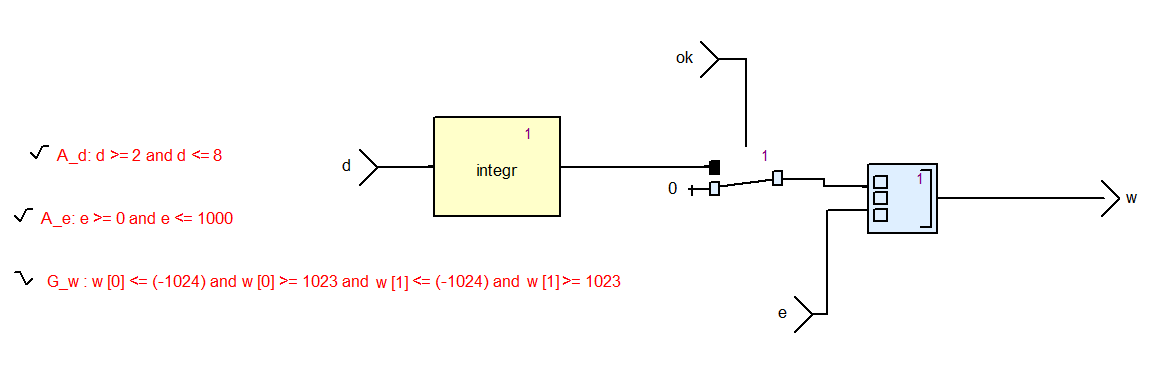
\includegraphics[scale=0.4]{4_extab.png}
\end{center}
\caption{Version graphique du noeud extab}
\end{figure}

\begin{figure}[h]
\begin{center}
\begin{small}
\begin{verbatim}
node extab(d : int; ok : bool; e : int) returns (w : int^2)
var
  _L1 : int;
  _L2 : int;
  _L3 : int;
  _L4 : bool;
  _L7 : int;
  _L8 : int^2;
  _L9 : int;
let
  _L1= #1 integr(_L2);
  _L2= d;
  _L3= if _L4 then (_L1) else (_L7);
  _L4= ok;
  _L7= 0;
  _L8= [_L3, _L9];
  _L9= e;
  w= _L8;
  assume A_d : d >= 2 and d <= 8;
  assume A_e : e >= -1023 and e <= 1024;
  guarantee G_w : w[0] <= - 1024 and w[0] >= 1023 and w[1] >= -1024 and
  w[1] <= 1023;
tel
\end{verbatim}
\end{small}
\end{center}
\caption{Version textuelle du noeud extab}
\end{figure}
\newpage
\noindent
Le couple de machines B engendré est le suivant:

\begin{center}
\begin{small}
\setlength{\columnseprule}{0.05cm}
\begin{multicols}{2}
\begin{alltt}
MACHINE Extab

OPERATIONS

ww \(\leftarrow\) extab(dd, ok, ee) =
 PRE
   ok \(\in\) BOOL &
   ee \(\in\) INT & ee >= 0 & ee <= 1000 &
   dd \(\in\) INT & dd >= 2 & dd <= 8
 THEN
   ww \(\in\): \{ ii | ii \(\in\) {0 .. 1} \(\rightarrow\) INT & 
      \(\forall\)jj. (jj \(\in\) {0 .. 1} \(\Rightarrow\) ii(jj) <= -1024 
      & ii(jj) >= 1023)\}
 END 
END
\end{alltt}
\columnbreak
\begin{alltt}
IMPLEMENTATION Extab_i
REFINES Extab

IMPORTS Integr

OPERATIONS

ww \(\leftarrow\) extab(dd, ok, ee) =
 VAR L1, L2, L3, L4, L7, L8, L9 IN
   L9 := ee; 
   L7 := 0; 
   L4 := ok; 
   L2 := dd; 
   L1 \(\leftarrow\) integr(L2); 
   IF L4=TRUE THEN L3 := L1 ELSE L3 := L7 END; 
   L8 := \{0 |-> L3, 1 |-> L9\}; 
   ww := L8
   
 END 
END

\end{alltt}
\end{multicols}
\end{small}
\end{center}

La définition d'un tableau est traduite par la définition d'une fonction B,
l'argument étant l'index du tableau, et la valeur renvoyée par la fonction correspond à la
valeur concernée du tableau.

\section*{Résumé}
Ces exemples représentent les différents mécanismes de traduction que l'on peut
rencontrer à partir du fragment de Scade considéré. Les machines produites sont
toutes correctes d'après l'analyse syntaxique et l'analyse de type de l'atelier B.
